\documentclass[12pt,aspectratio=169,UTF8]{ctexbeamer}

% ===== 主题 =====
\usetheme{Madrid}
\usecolortheme{default}
\usefonttheme{professionalfonts}
\graphicspath{{images/}}

% ===== 颜色 =====
\definecolor{primary}{HTML}{5B7FFF}
\definecolor{accent}{HTML}{00C897}
\definecolor{warn}{HTML}{F59E0B}
\definecolor{danger}{HTML}{FF6B6B}
\definecolor{bg}{HTML}{F0F2F5}

\setbeamercolor{structure}{fg=primary}
\setbeamercolor{frametitle}{fg=white,bg=primary}
\setbeamercolor{block title}{fg=white,bg=primary}
\setbeamercolor{block body}{fg=black,bg=bg}
\setbeamercolor{alerted text}{fg=danger}
\setbeamercolor{example text}{fg=accent}
\setbeamercolor{palette primary}{fg=white,bg=primary}
\setbeamertemplate{items}[circle]
\setbeamertemplate{navigation symbols}{}

% ===== 标题页 =====
\title{个人记账系统}
\subtitle{MyMoneyBook —— 进展报告}
\author{王偲哲 \quad 2500017779}
\institute{程序设计实习 \quad 指导教师：贾川民}
\date{2026年6月6日}

\begin{document}

% ==================== 标题页 ====================
\begin{frame}
  \titlepage
\end{frame}

% ==================== 项目概述 ====================
\section{项目概述}

\begin{frame}{项目概述}
  \begin{columns}[t]
    \column{0.48\textwidth}
    \begin{block}{项目定位与技术栈}
      \begin{itemize}
        \item 基于 Qt6 的桌面个人记账软件
        \item C++17 + Qt 6.11（Widgets/Sql/Charts）
        \item SQLite 本地数据存储，CMake 构建
        \item 三层架构：Widget → 业务逻辑 → 数据访问层
      \end{itemize}
    \end{block}

    \column{0.52\textwidth}
    \begin{block}{已实现功能（8 项）}
      \begin{enumerate}
        \item 用户注册与登录（SHA-256 加盐哈希）
        \item 账单 CRUD + CSV 导出
        \item 分类管理（15 个预置分类）
        \item 预算管理（三级变色预警）
        \item 多条件搜索筛选 + 汇总
        \item 饼图 + 折线图可视化
        \item 全局 QSS 主题（280+ 行）
        \item 数据库外键约束 + 余额联动
      \end{enumerate}
    \end{block}
  \end{columns}
\end{frame}

% ==================== 登录与注册 ====================
\section{登录与注册}

\begin{frame}{登录与注册}
  \begin{columns}[t]
    \column{0.48\textwidth}
    \begin{block}{功能要点}
      \begin{itemize}
        \item QStackedWidget 切换登录/注册页
        \item 密码 SHA-256 加盐哈希存储
        \item 注册验证：用户名 $\ge$ 3 字符，密码 $\ge$ 4 字符
        \item 注册后自动创建默认账户 \& 15 个分类
      \end{itemize}
    \end{block}
    \vspace{6pt}
    \centering
    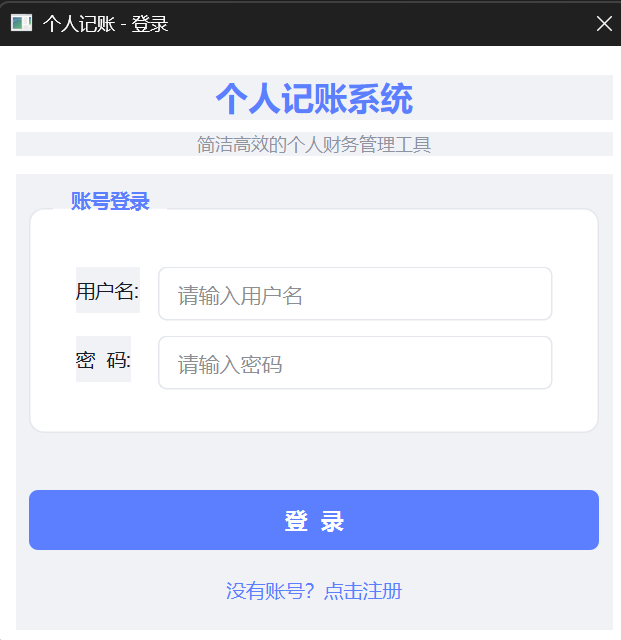
\includegraphics[width=0.85\textwidth]{登录界面.png}

    \column{0.52\textwidth}
    \centering
    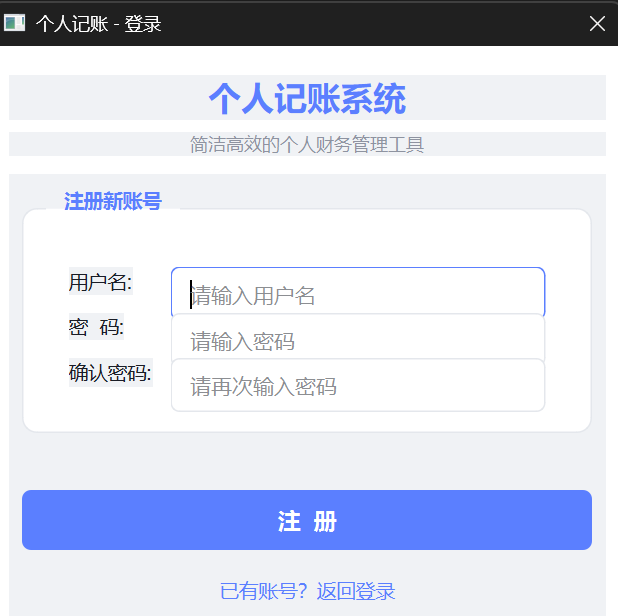
\includegraphics[width=0.90\textwidth]{注册界面.png}
  \end{columns}
\end{frame}

% ==================== 账单管理 ====================
\section{账单管理}

\begin{frame}{账单管理}
  \begin{columns}[t]
    \column{0.48\textwidth}
    \begin{block}{功能要点}
      \begin{itemize}
        \item 收支记录的增删改，按时间倒序展示
        \item 类型切换自动联动过滤分类
        \item 顶部实时汇总收入/支出/结余
        \item CSV 一键导出全部账单
        \item 金额列按收支类型着色
      \end{itemize}
    \end{block}
    \vspace{6pt}
    \centering
    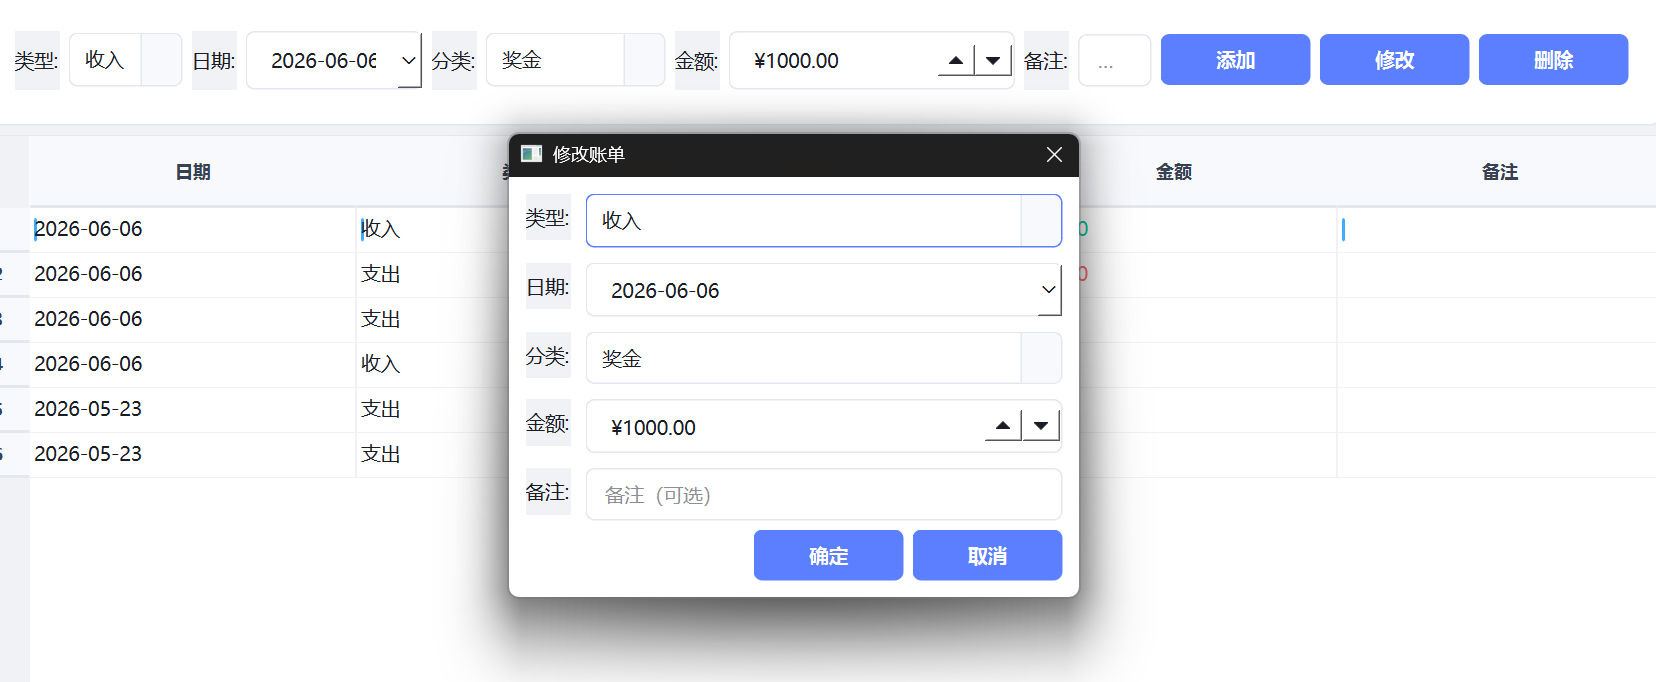
\includegraphics[width=0.85\textwidth]{修改账目.png}

    \column{0.52\textwidth}
    \centering
    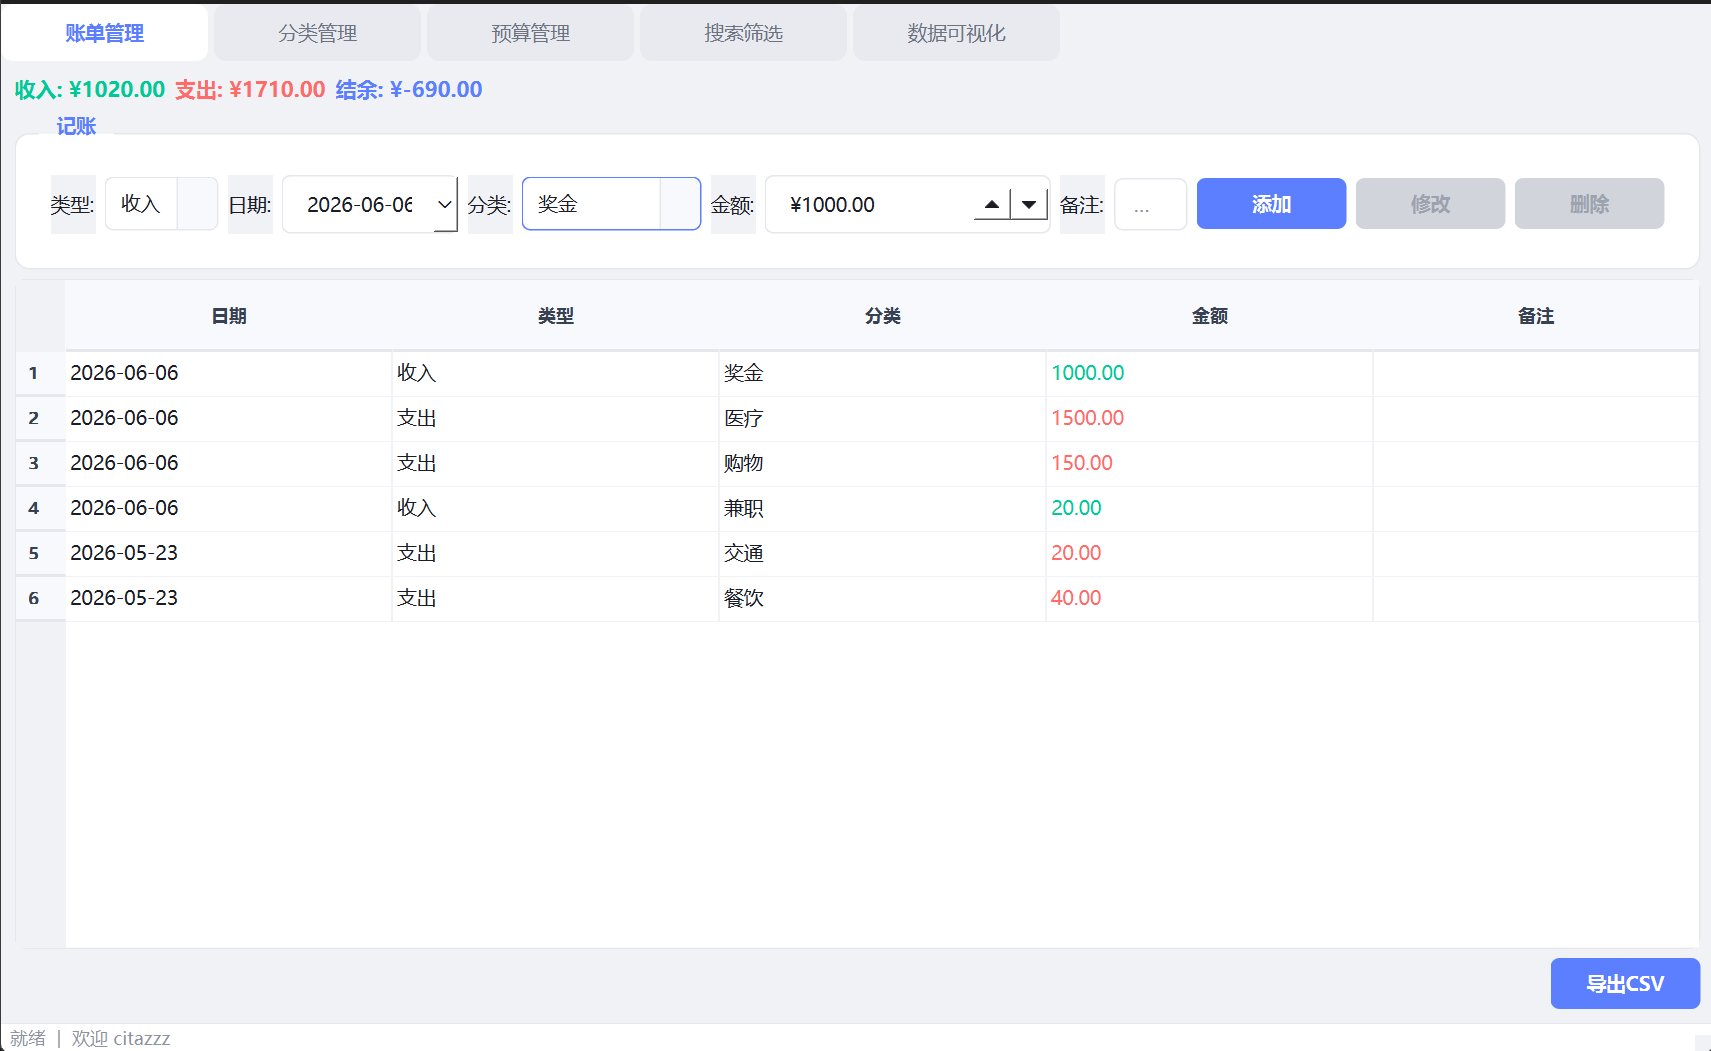
\includegraphics[width=\textwidth]{账单界面.png}
  \end{columns}
\end{frame}

% ==================== 分类与预算 ====================
\section{分类管理 \& 预算管理}

\begin{frame}{分类管理 \& 预算管理}
  \begin{columns}[t]
    \column{0.48\textwidth}
    \begin{block}{分类管理}
      \begin{itemize}
        \item 预置 5 收入 + 10 支出分类
        \item 支持自定义增删改
        \item 收入/支出分色显示
      \end{itemize}
    \end{block}

    \begin{block}{预算管理}
      \begin{itemize}
        \item 按月设置支出预算
        \item 实时统计已支出 / 剩余
        \item 三级变色预警：\\
        {\color{accent} $<\!80\%$ 绿色} $\cdot$ {\color{warn}$80\!\sim\!100\%$ 橙色} $\cdot$ {\color{danger}$>\!100\%$ 红色}
        \item 账单变更后自动刷新
      \end{itemize}
    \end{block}

    \column{0.52\textwidth}
    \centering
    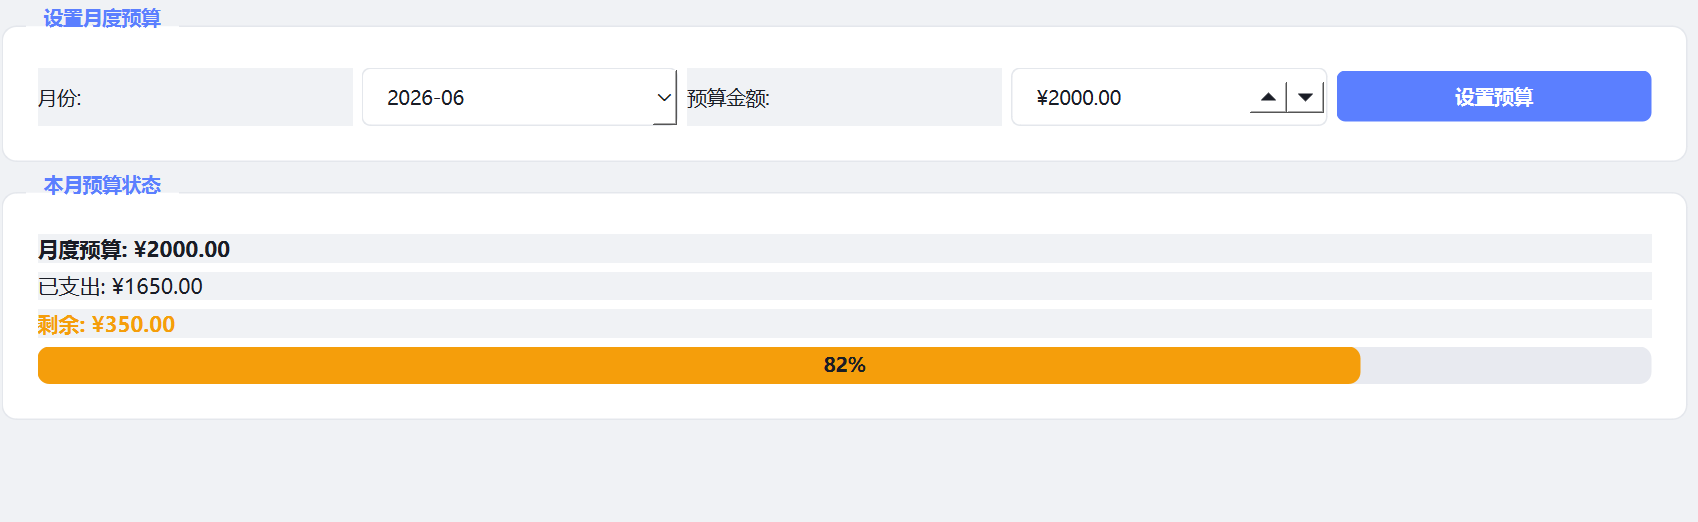
\includegraphics[width=\textwidth]{预算界面.png}
    \vspace{6pt}
    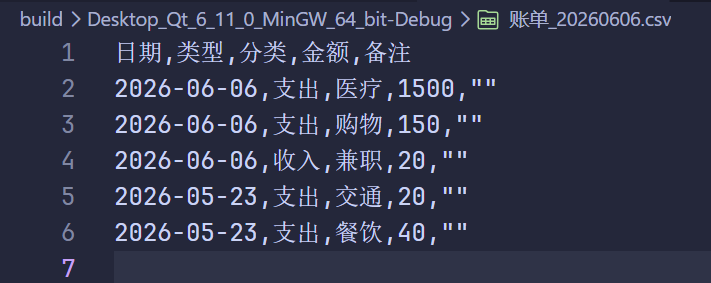
\includegraphics[width=0.60\textwidth]{导出csv.png}
  \end{columns}
\end{frame}

% ==================== 搜索筛选 & 数据可视化 ====================
\section{搜索筛选 \& 数据可视化}

\begin{frame}{搜索筛选 \& 数据可视化}
  \begin{columns}[t]
    \column{0.48\textwidth}
    \begin{block}{多条件搜索}
      \begin{itemize}
        \item 关键字模糊搜索备注
        \item 收支类型 / 分类 / 日期范围组合筛选
        \item 结果底部自动汇总（灰底高亮）
        \item 一键重置条件
      \end{itemize}
    \end{block}

    \begin{block}{数据可视化}
      \begin{itemize}
        \item \textbf{饼图}：分类占比 + 百分比标签
        \item \textbf{折线图}：每日收支趋势
        \item 自由切换收支类型和时间范围
      \end{itemize}
    \end{block}

    \column{0.52\textwidth}
    \centering
    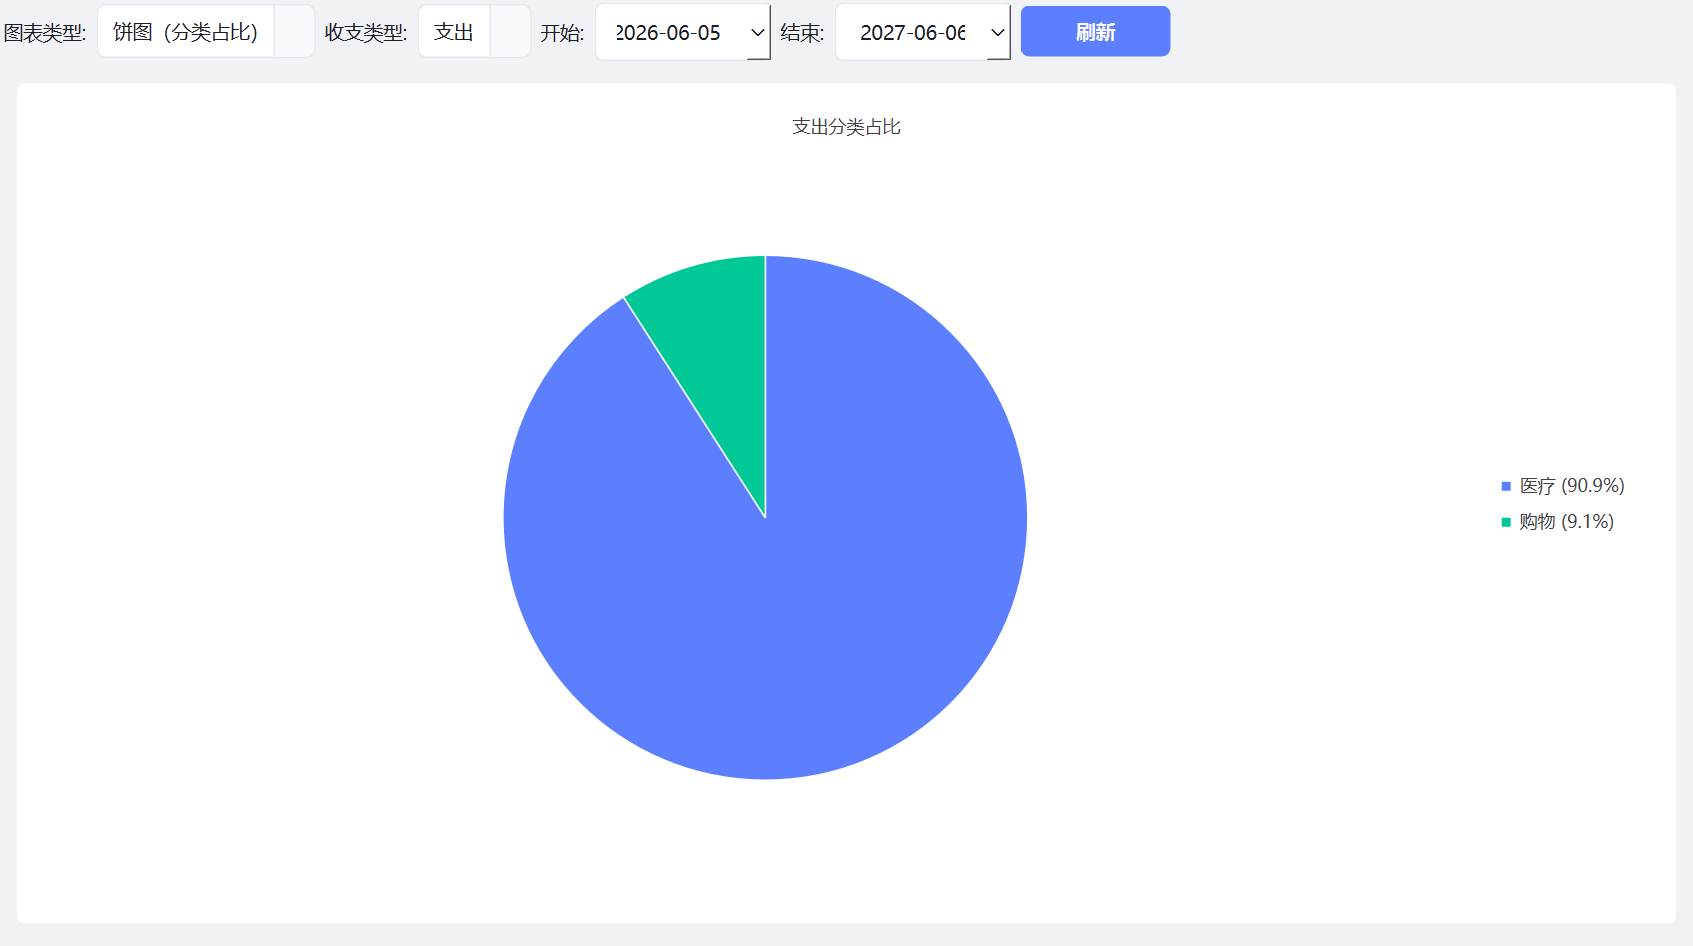
\includegraphics[width=\textwidth]{统计饼图.png}
  \end{columns}
\end{frame}

% ==================== 类设计 ====================
\section{类设计}

\begin{frame}[fragile]{类设计概览}
  \small
  \begin{columns}[t]
    \column{0.45\textwidth}
    \begin{block}{核心类}
      \begin{tabular}{ll}
        \textbf{databaseManager} & 单例，SQLite 数据访问层 \\
        \textbf{LoginDialog}     & 登录/注册对话框 \\
        \textbf{MainWindow}      & QTabWidget 管理 5 页 \\
        \textbf{BillWidget}      & 账单 CRUD + CSV 导出 \\
        \textbf{CategoryManager} & 收支分类管理 \\
        \textbf{BudgetWidget}    & 月度预算 + 变色预警 \\
        \textbf{SearchFilter}    & 多条件组合筛选 \\
        \textbf{Visualization}   & 饼图 + 折线图 \\
      \end{tabular}
    \end{block}

    \column{0.55\textwidth}
    \begin{block}{协作关系}
\begin{verbatim}
main.cpp
  ├── LoginDialog → databaseManager
  └── MainWindow
        ├── BillWidget → DB
        │     └── billsChanged() → BudgetWidget
        ├── CategoryManager → DB
        ├── BudgetWidget → DB
        ├── SearchFilter → DB
        └── Visualization → DB
\end{verbatim}
    \end{block}
  \end{columns}

  \vspace{6pt}
  \begin{center}
    \small
    数据库 5 表：\texttt{users} $\cdot$ \texttt{accounts} $\cdot$ \texttt{categories} $\cdot$ \texttt{bills} $\cdot$ \texttt{budgets}
    \quad 全部通过外键关联，\texttt{ON DELETE CASCADE} 保证完整性
  \end{center}
\end{frame}

% ==================== 开发进展与差异 ====================
\section{开发进展与差异}

\begin{frame}{开发进展与差异}
  \begin{columns}[t]
    \column{0.48\textwidth}
    \begin{alertblock}{待集成：多账户管理}
      AccountManagerWidget 代码已完成，待：
      \begin{itemize}
        \item 数据库 API 补充
        \item CMake 编译配置更新
        \item 主界面 Tab 挂载
        \item 账单页增加账户选择
      \end{itemize}
    \end{alertblock}

    \begin{block}{主要差异}
      \begin{itemize}
        \item 多账户管理：代码已写，未集成
        \item 分类图标：未实现
        \item 可视化为自定义日期范围（更灵活）
        \item 预算预警三级变色（超出设计预期）
      \end{itemize}
    \end{block}

    \column{0.52\textwidth}
    \begin{exampleblock}{完成度：约 85\%}
      \textbf{已完成}：登录注册、账单 CRUD、分类管理、预算预警、多条件筛选、饼图+折线图、CSV导出、QSS主题

      \vspace{6pt}
      \textbf{待完成}：账户管理集成、分类图标
    \end{exampleblock}

    \vspace{6pt}
    \begin{block}{技术收获}
      Qt 信号槽机制、Model/View 架构、SQLite 外键设计、单例模式、完整桌面应用开发流程
    \end{block}
  \end{columns}
\end{frame}

% ==================== 致谢 ====================
\begin{frame}
  \begin{center}
    \Huge
    {\color{primary}谢谢！}

    \vspace{24pt}
    \normalsize
    个人记账系统 \quad MyMoneyBook

    \vspace{8pt}
    \small
    Qt6 \;/\; C++17 \;/\; SQLite \;/\; CMake
  \end{center}
\end{frame}

\end{document}
